% Appendix1 file from standard thesis template

\appendixtitle 
\appendix

%% Use the following two lines for single appendix
\unappendixtitle
\singleappendixtitle

% \chapter{ADDITIONAL MATERIAL} 

\begin{figure}
    \centering
    \begin{minipage}{0.49\textwidth}
        \centering
        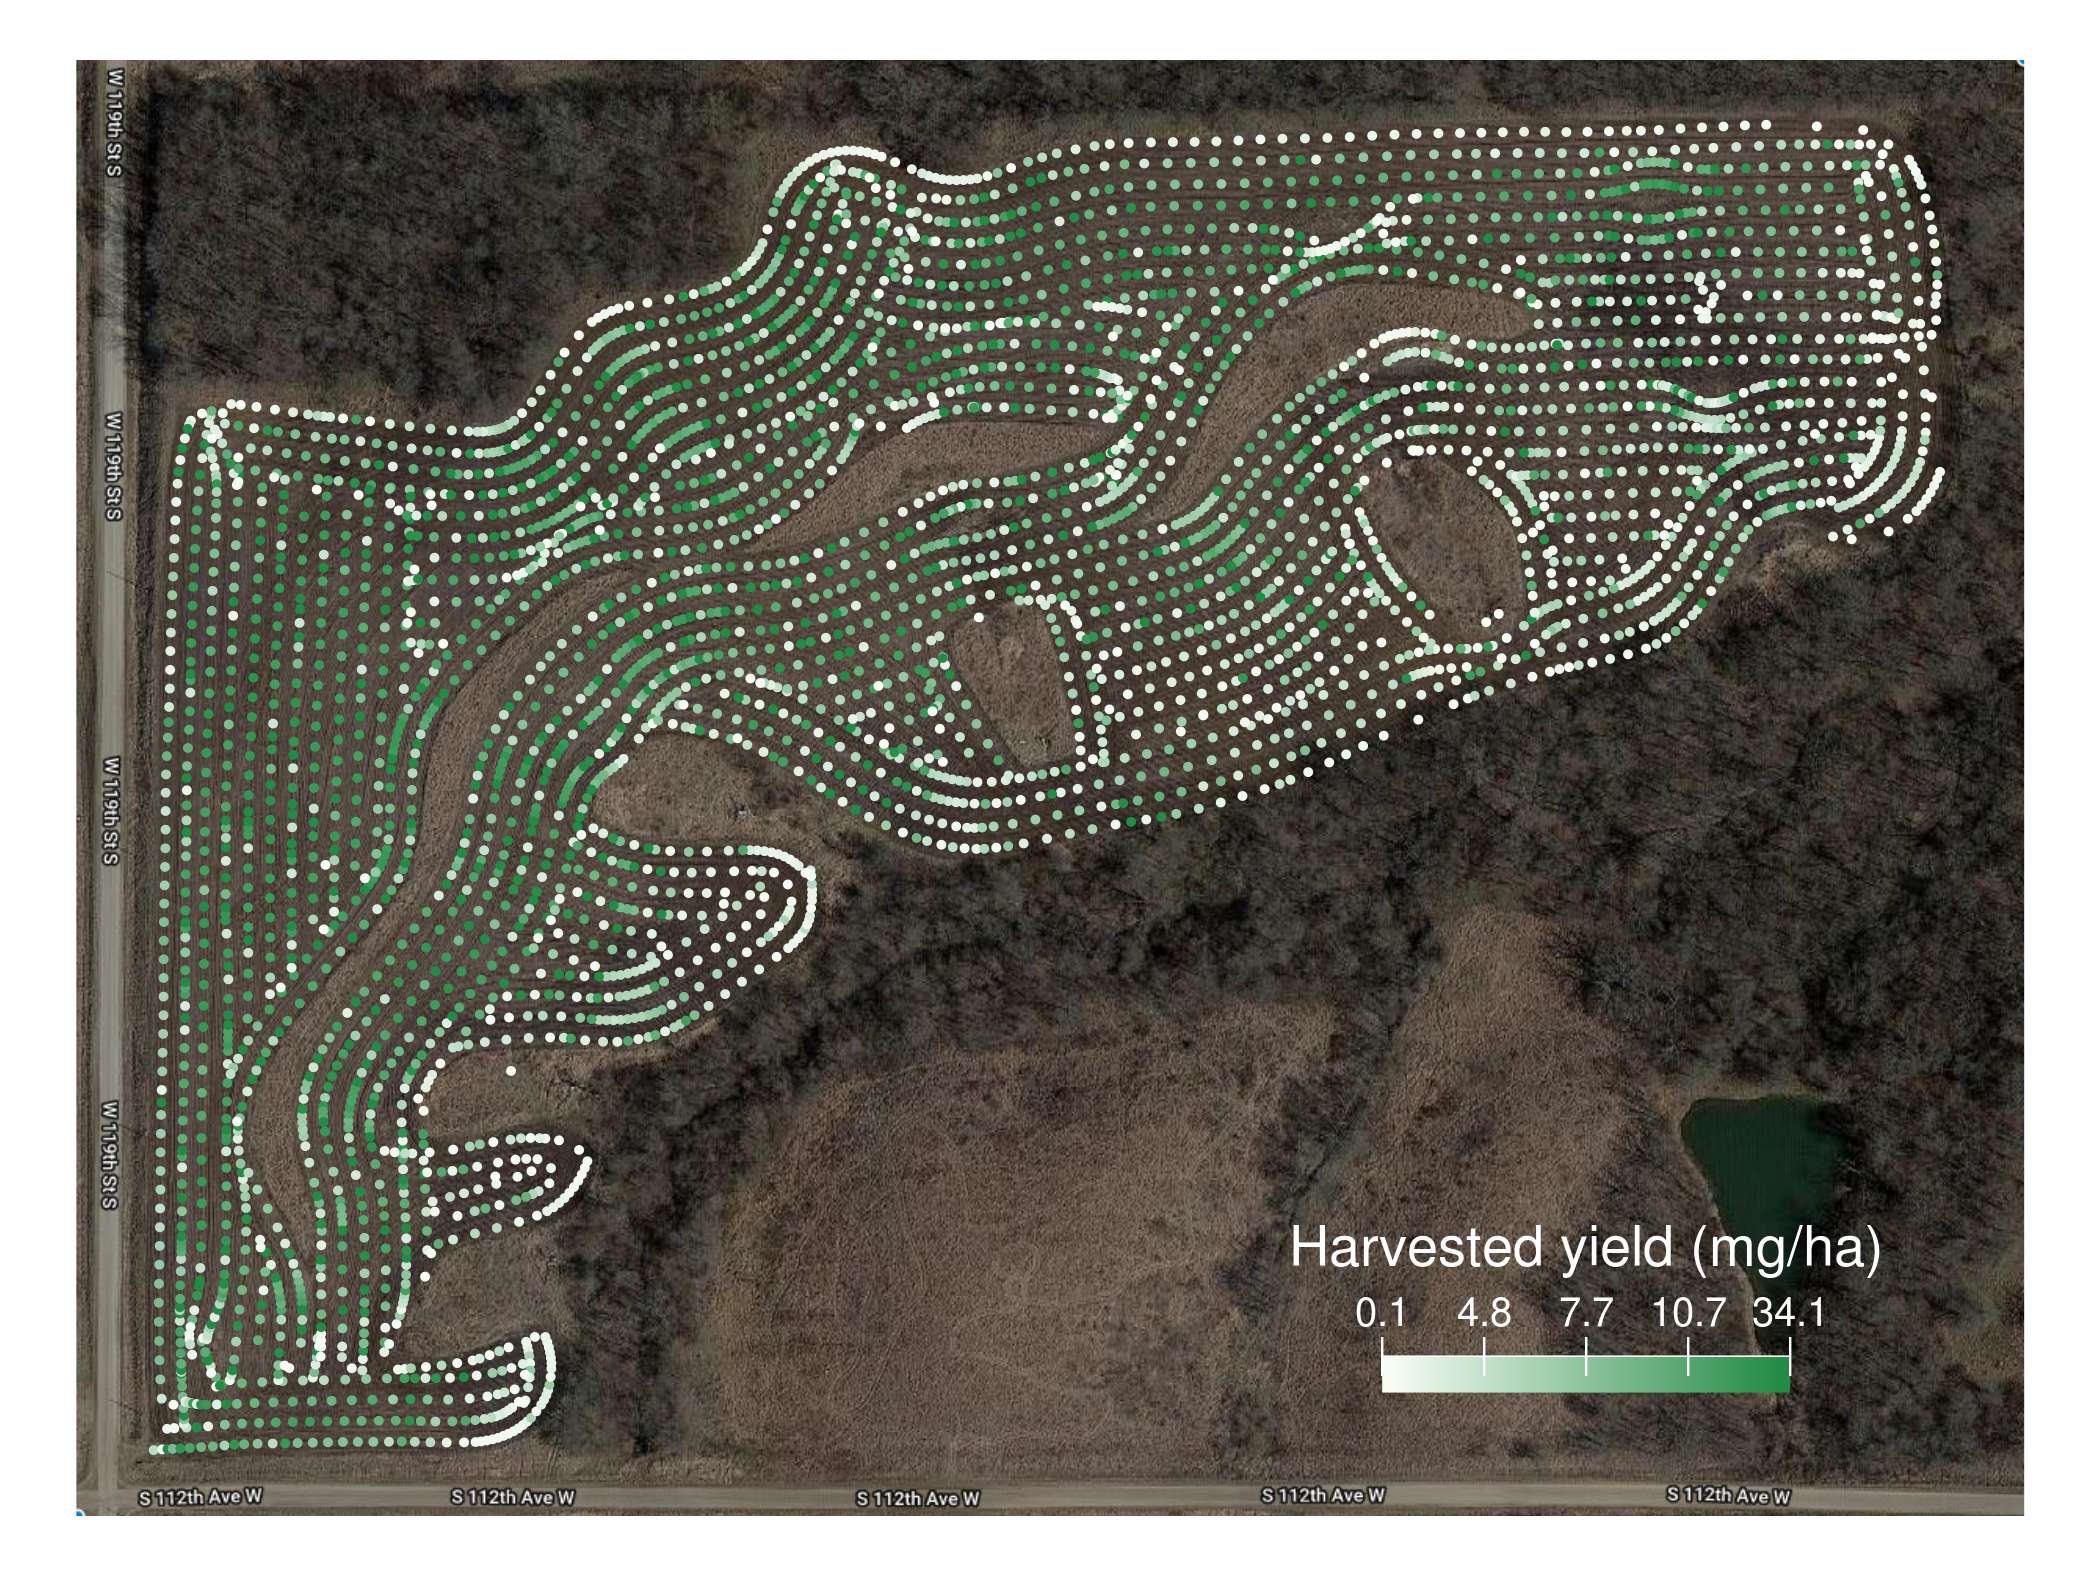
\includegraphics[width=0.75\textwidth]{appendix/basswood_2012_res5_1_points_vehicle}
        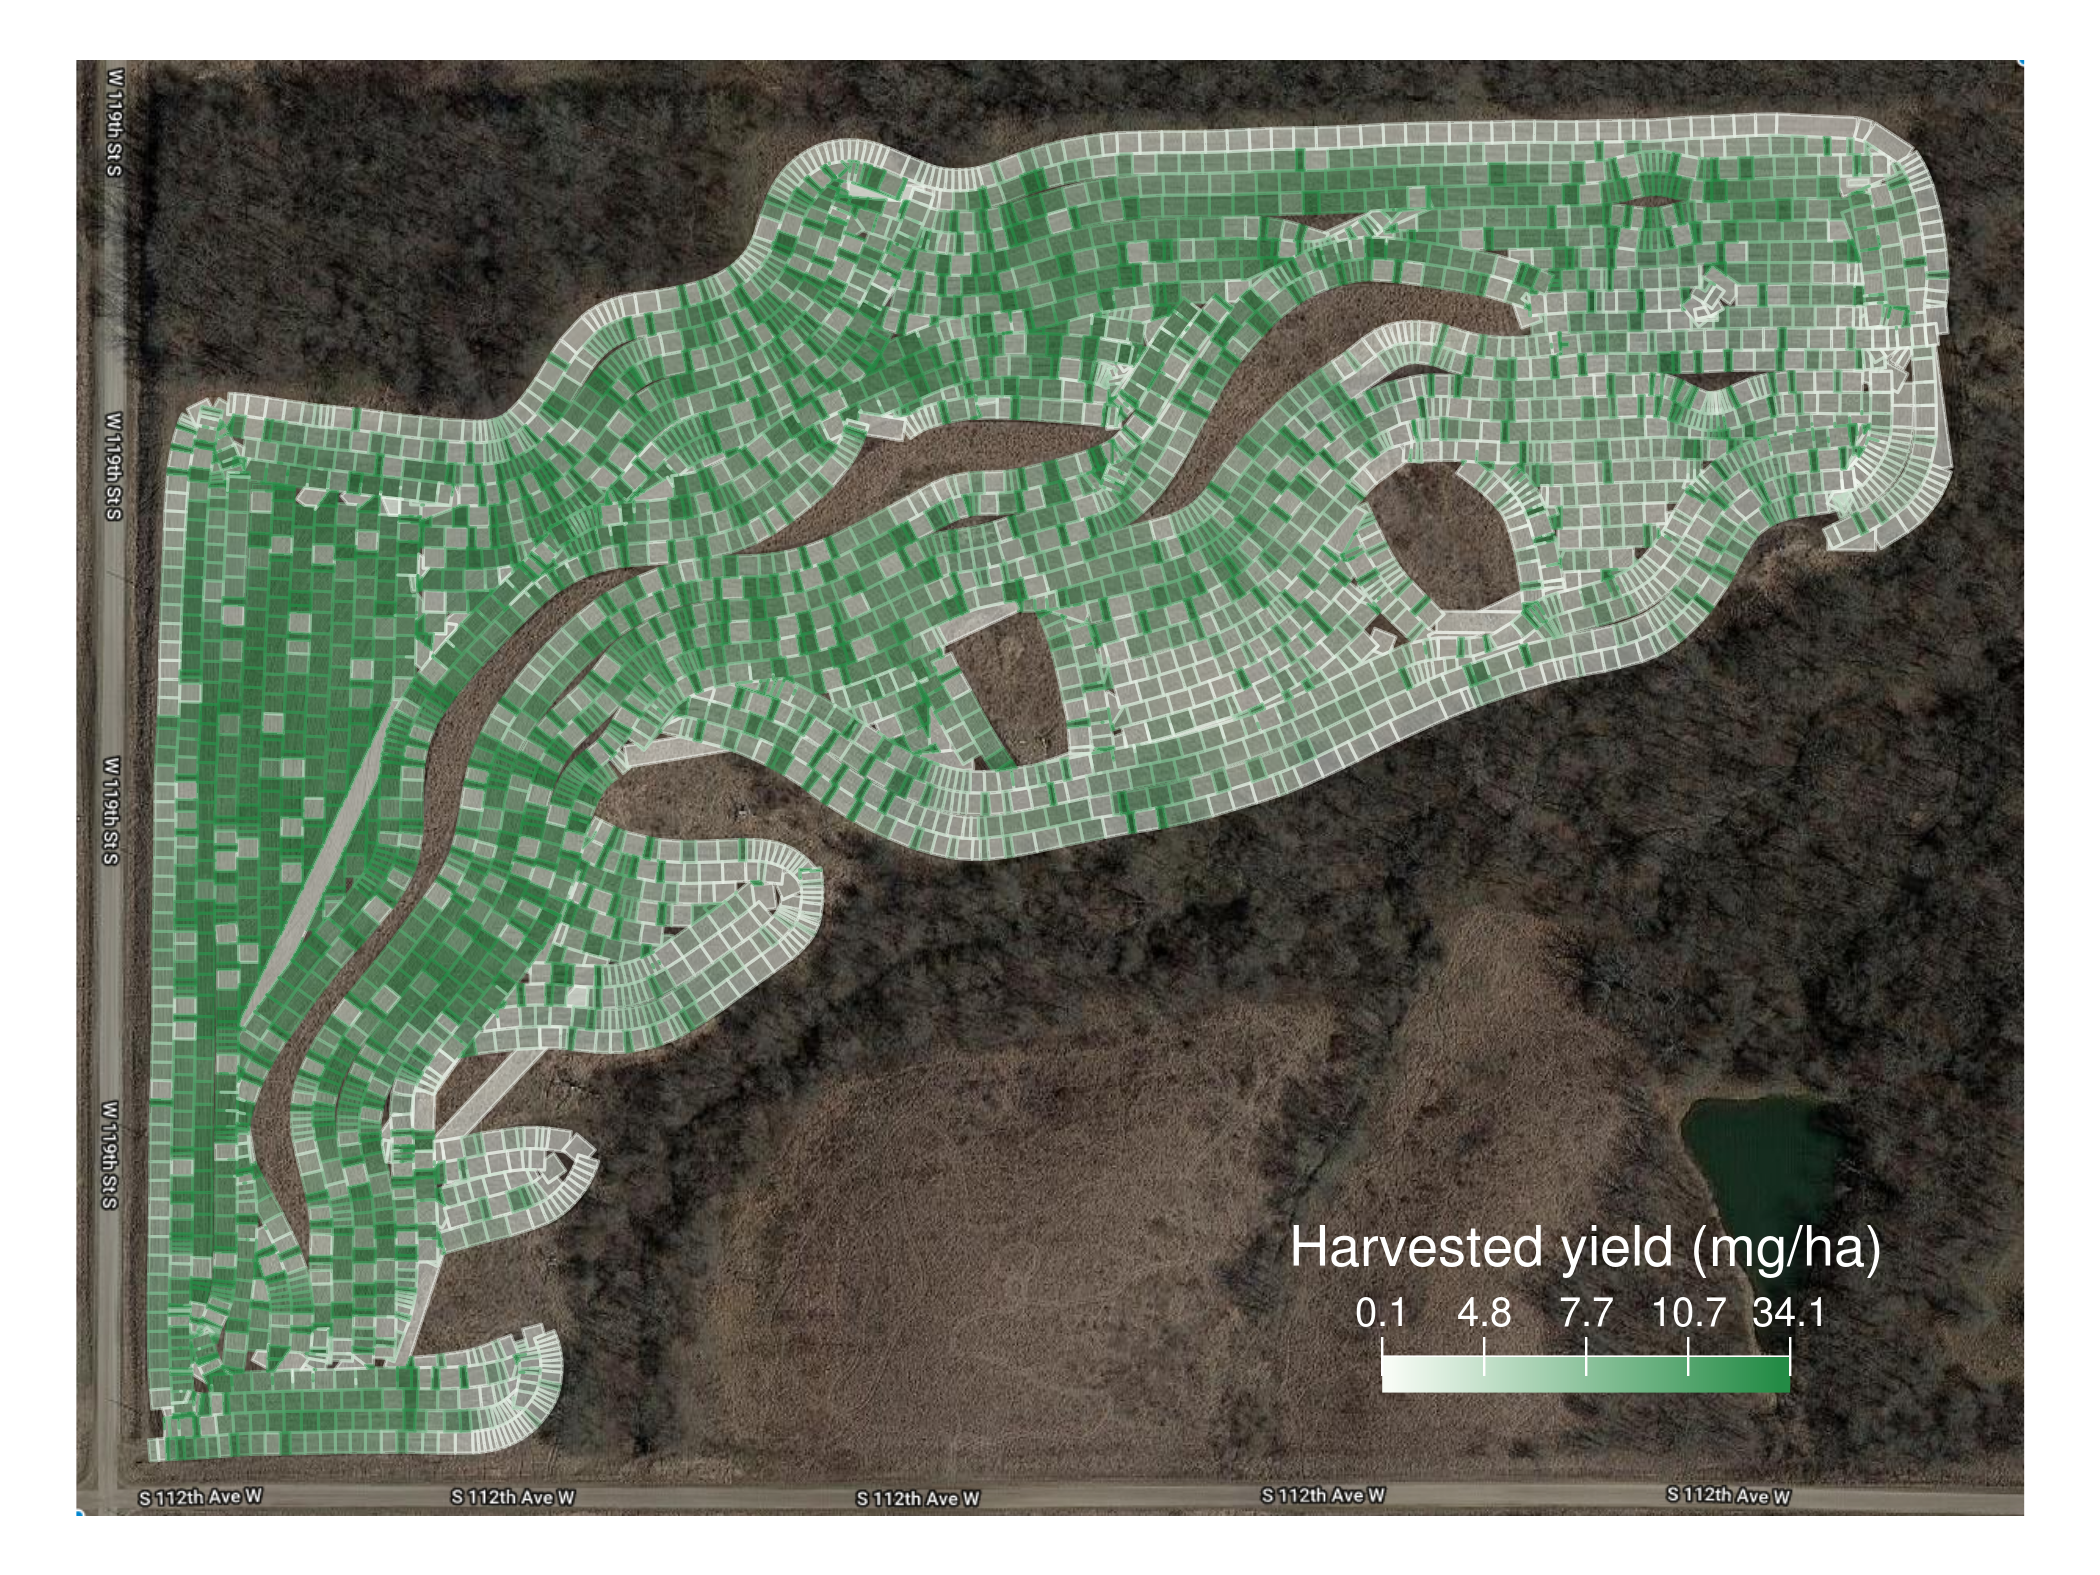
\includegraphics[width=0.75\textwidth]{appendix/basswood_2012_res5_1_reshaped}
        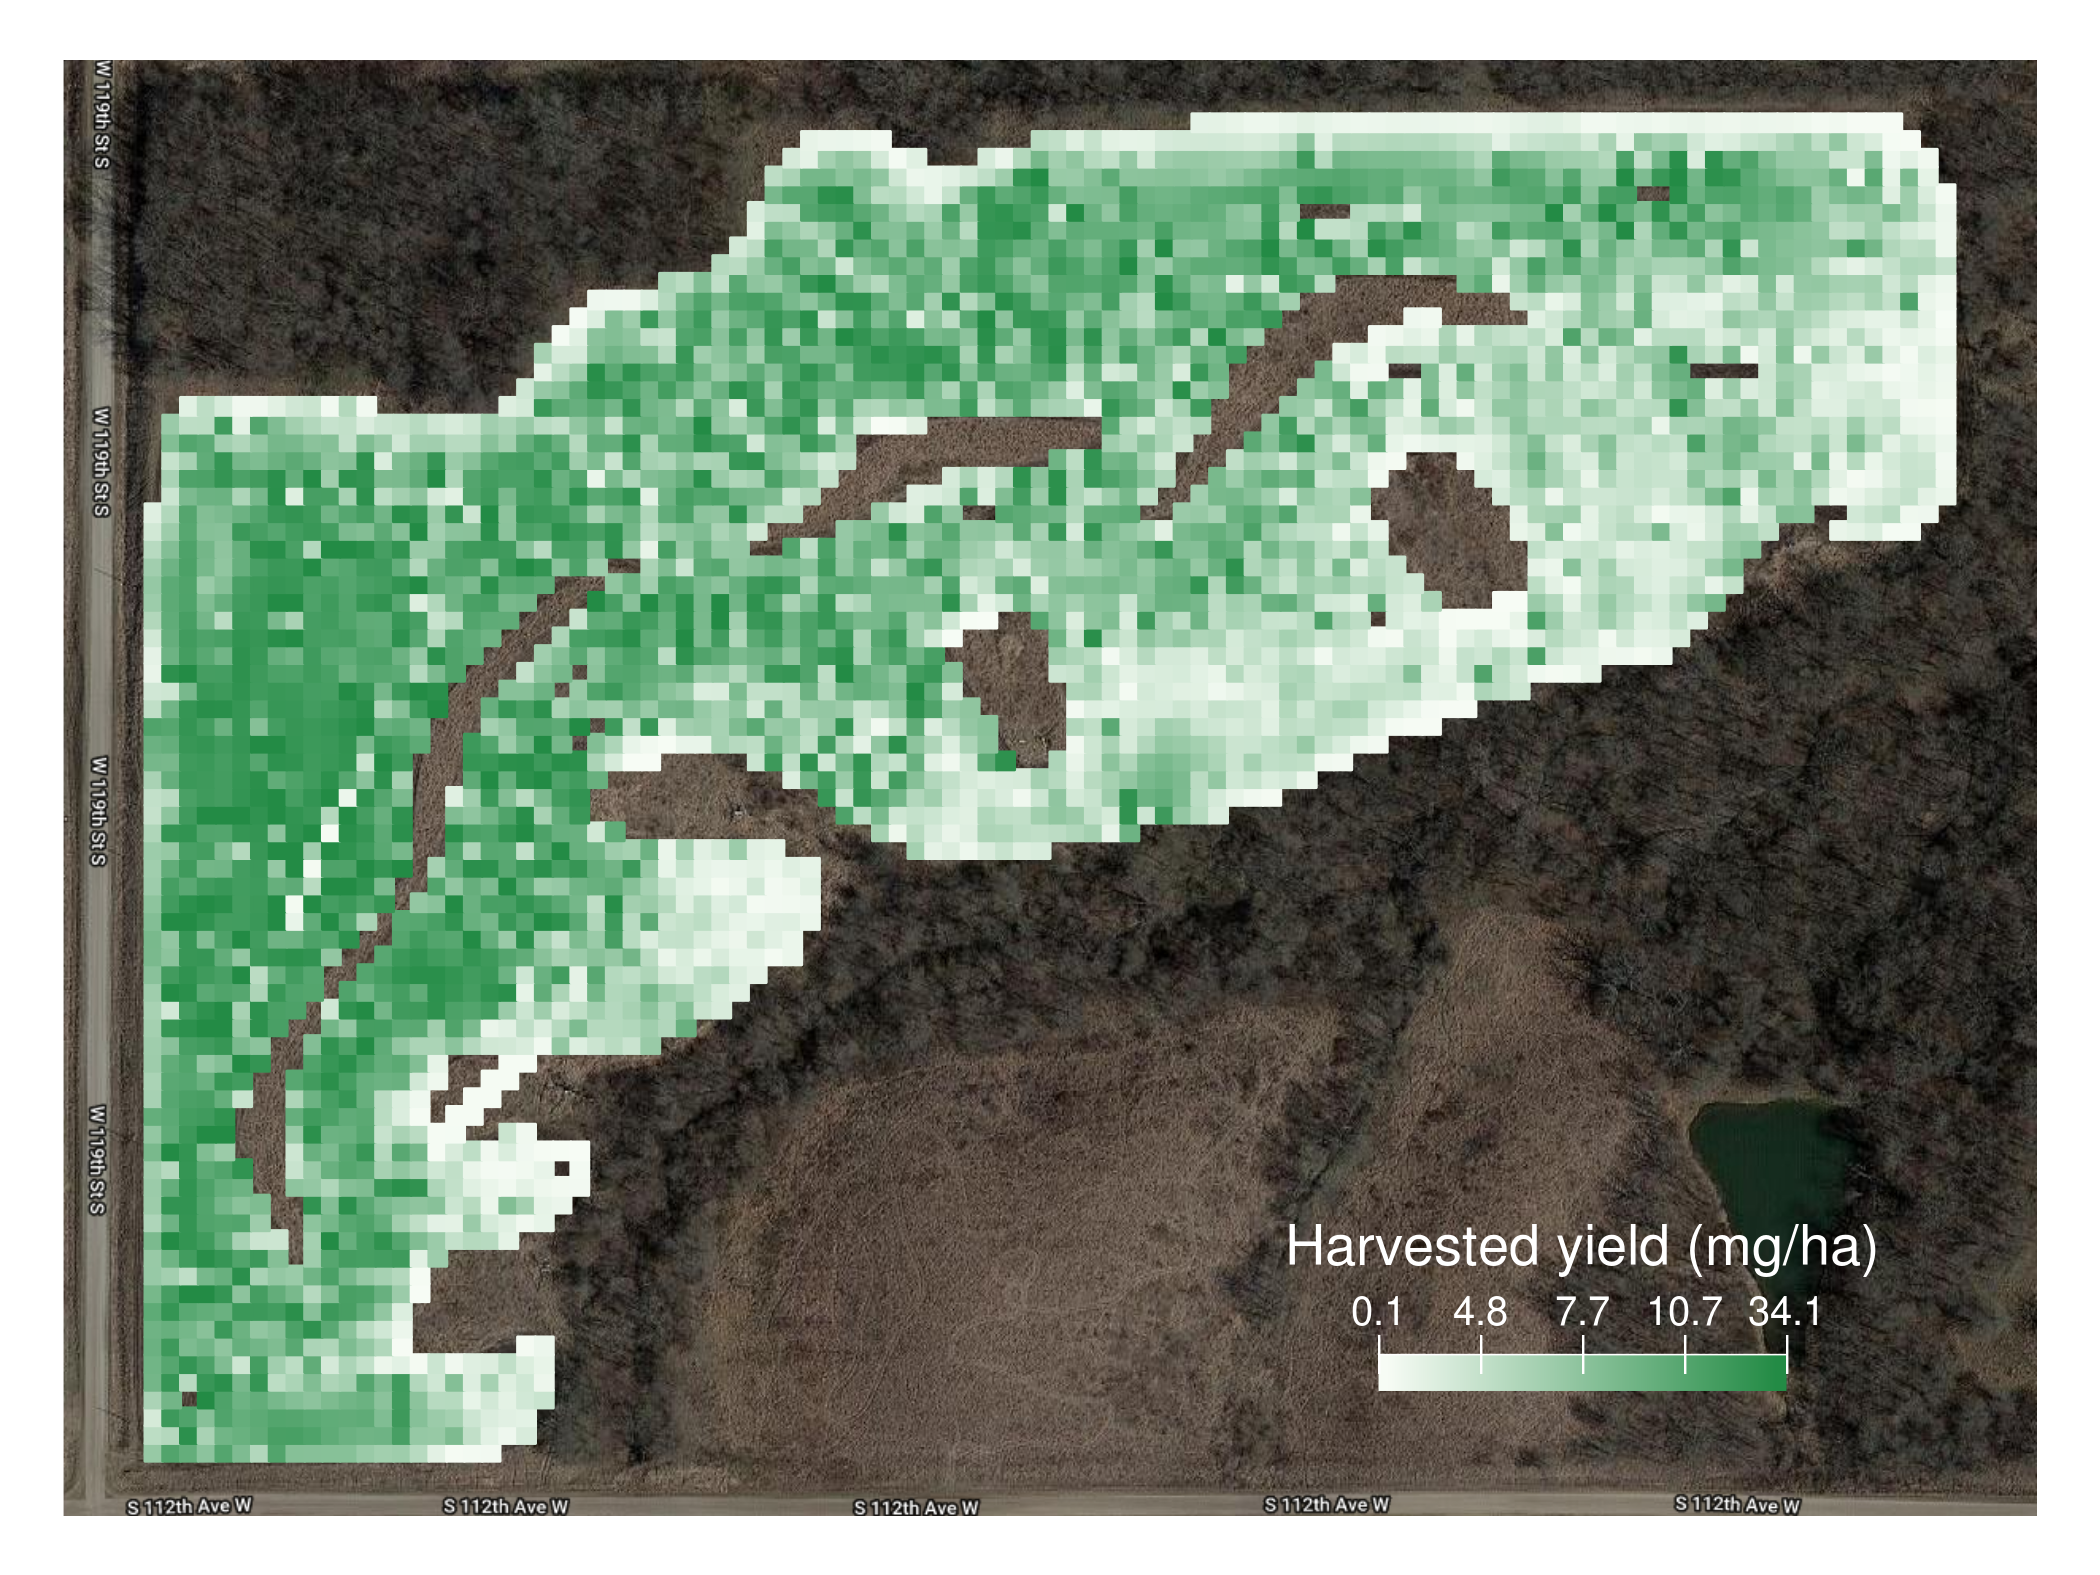
\includegraphics[width=0.75\textwidth]{appendix/basswood_2012_res5_1_aggregated}
    \end{minipage}\hfill
    \begin{minipage}{0.49\textwidth}
        \centering
        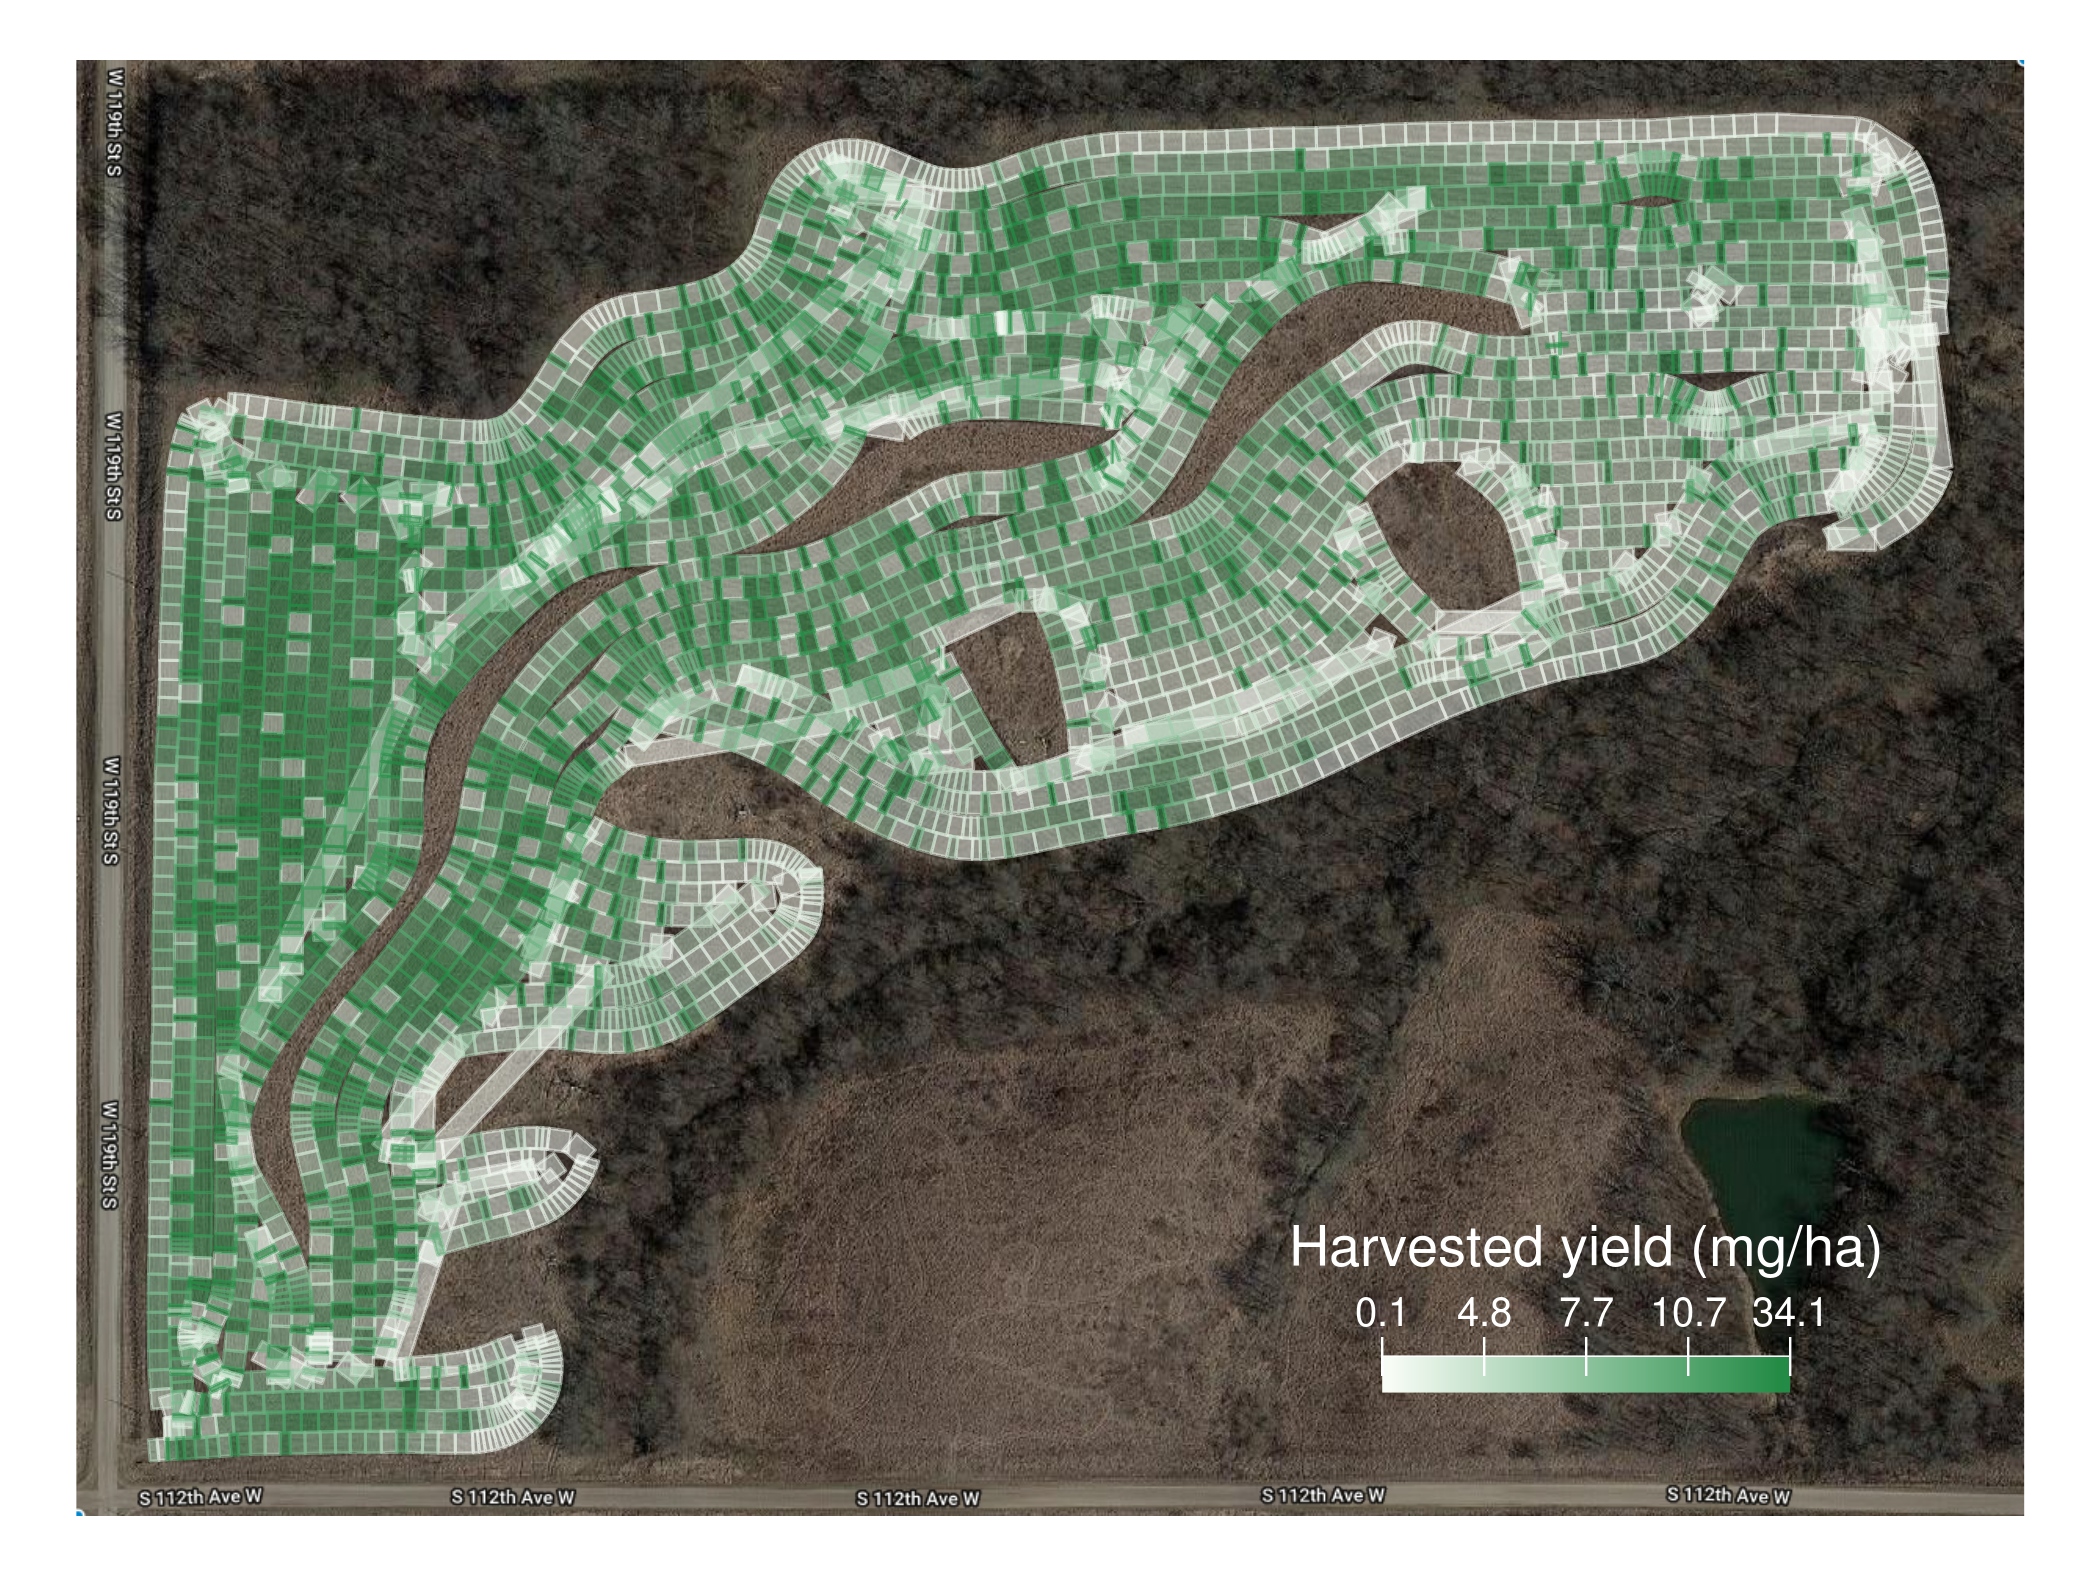
\includegraphics[width=0.75\textwidth]{appendix/basswood_2012_res5_1_polygons_vehicle}
        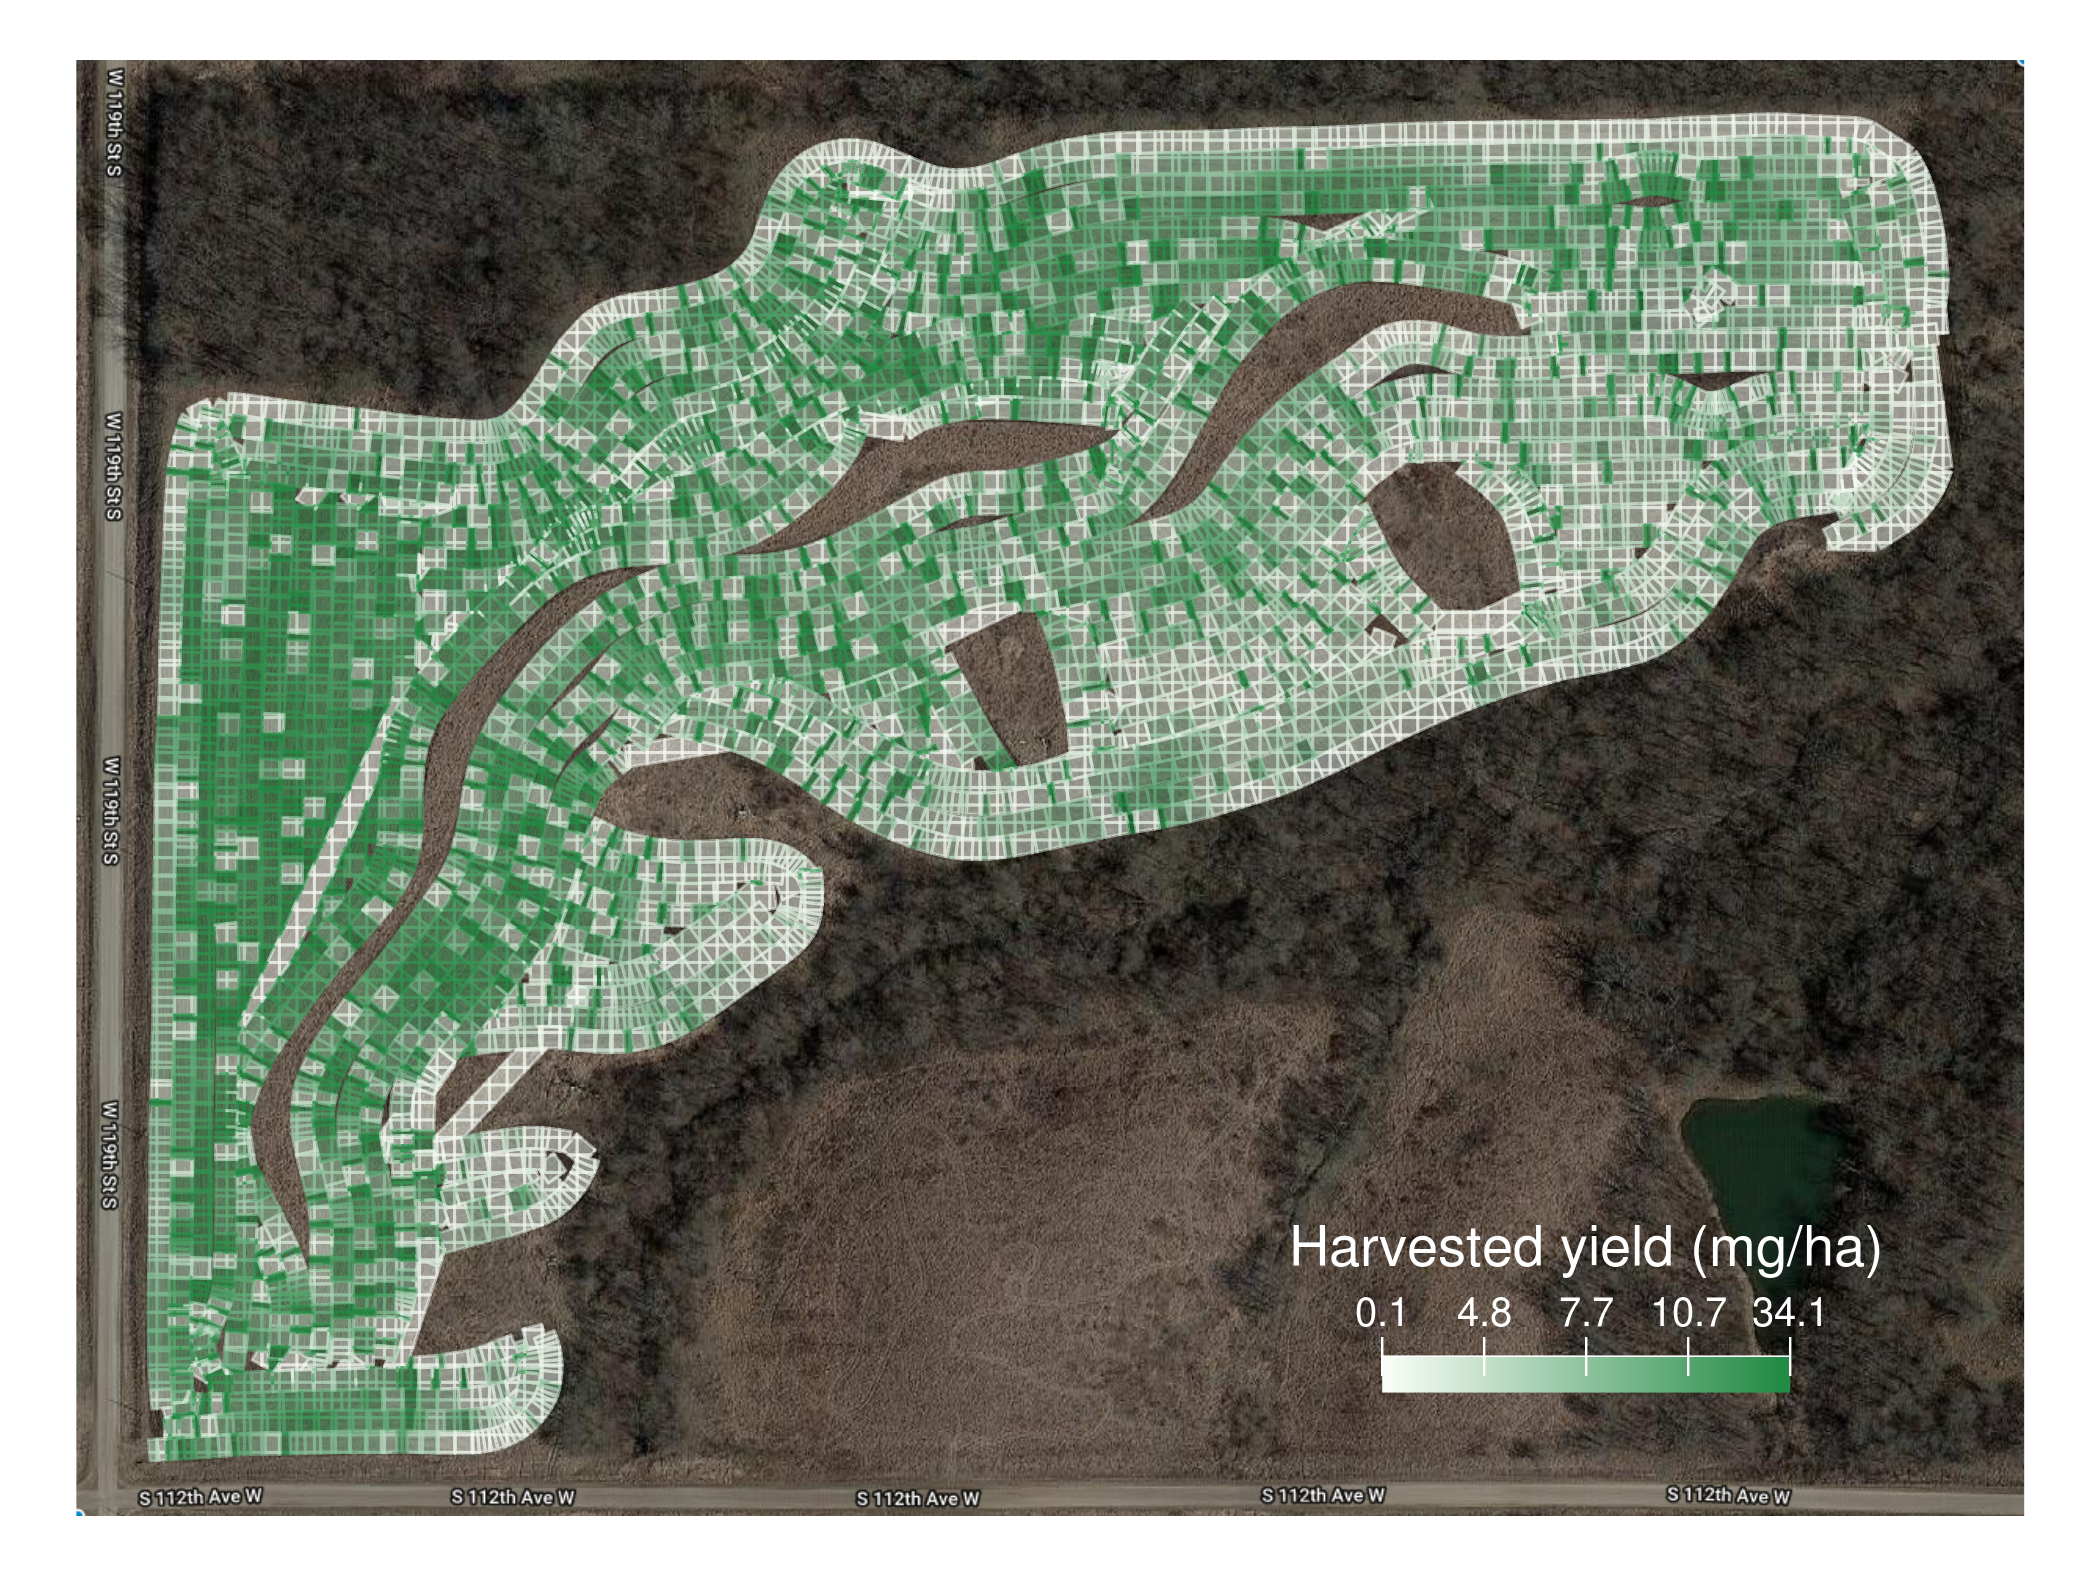
\includegraphics[width=0.75\textwidth]{appendix/basswood_2012_res5_1_chopped}
        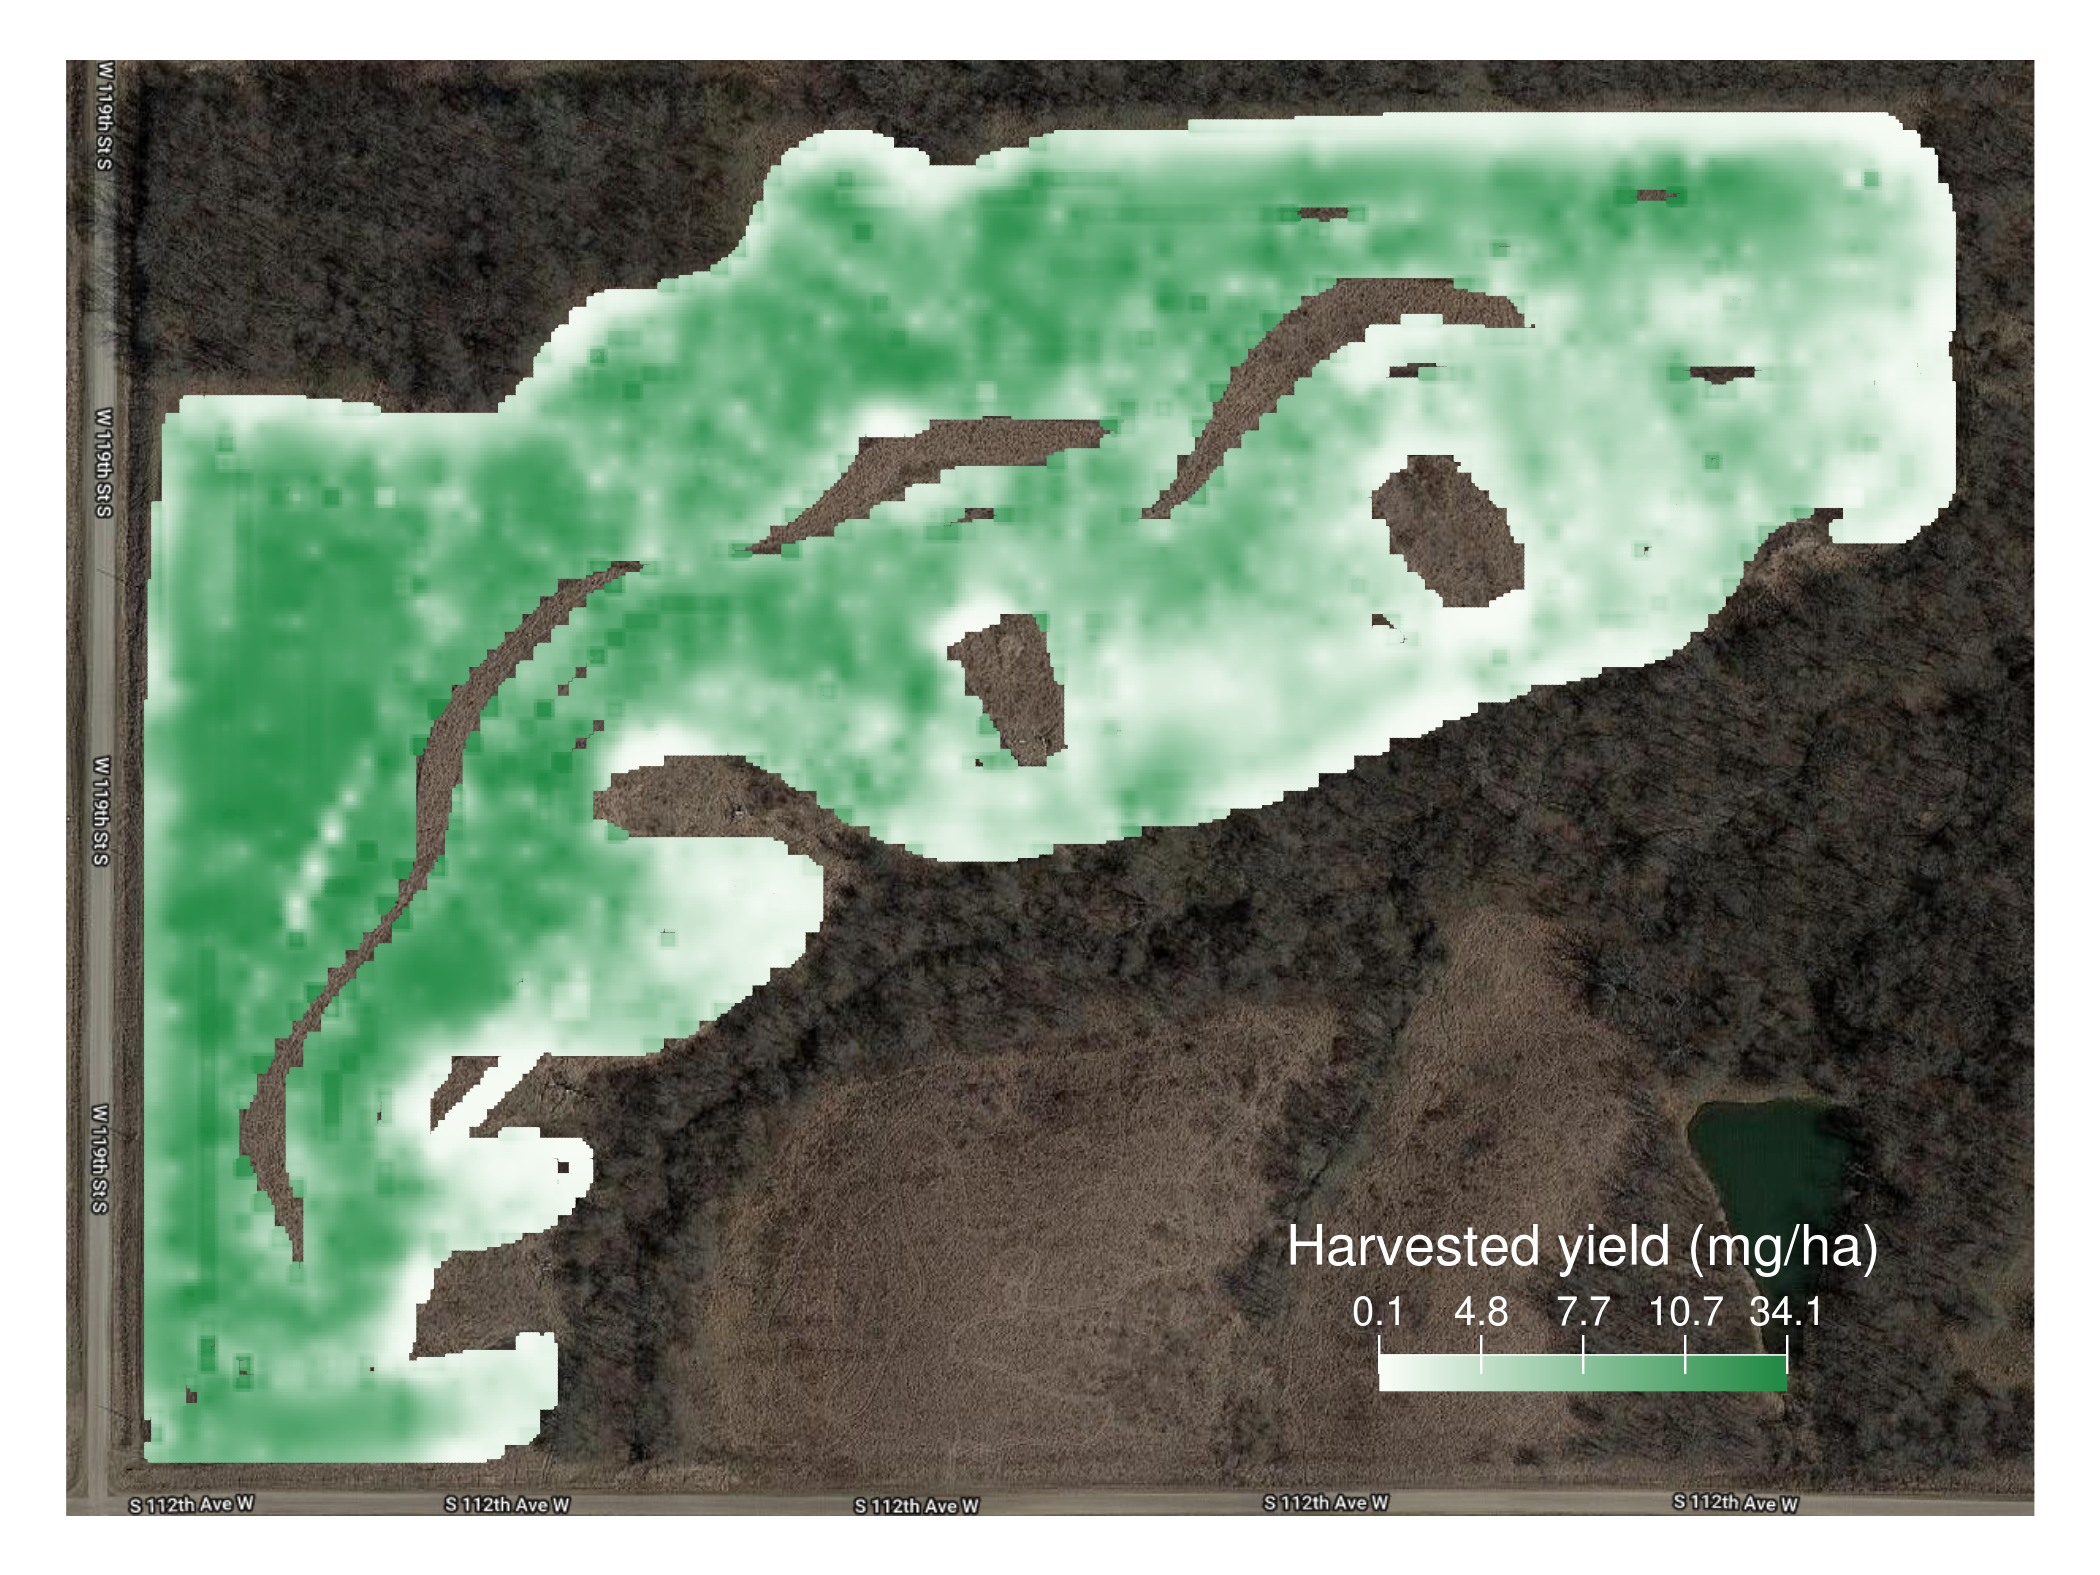
\includegraphics[width=0.75\textwidth]{appendix/basswood_2012_res5_1_smoothed}
    \end{minipage}
    \caption[Step-by-step visualization of the algorithm for one field]{Every step progression. Point and intersection maps
      in the top row, reshaped and clipped maps in the middle row, and
    aggregated and smooth maps in the bottom row.}
    \label{fig:basswood2012-all-steps}
\end{figure}

%%% Local Variables:
%%% mode: latex
%%% TeX-master: "../thesis"
%%% End:
